\documentclass[conference]{IEEEtran}
%\usepackage{spconf,amsmath,amssymb,graphicx}
\usepackage{amsmath,amssymb,graphicx,caption,listings,hyperref,graphicx,verbatim}

% Example definitions.
% --------------------
% nice symbols for real and complex numbers
\newcommand{\R}[0]{\mathbb{R}}
\newcommand{\C}[0]{\mathbb{C}}
% bold paragraph titles
\newcommand{\mypar}[1]{{\bf #1.}}
\newcommand{\mysubpar}[2]{{\bf #1.}}
\graphicspath{ {./images/} }

\lstset{frame=tb,
  language=C,
  aboveskip=5mm,
  belowskip=5mm,
  showstringspaces=true,
  columns=flexible,
  numbers=none,	
  breaklines=true,
  breakatwhitespace=true,
  tabsize=2
}

\begin{document}

\title{The Reinforcement Learning for Structural Evolution method on a Docker Environment}


\author{\IEEEauthorblockN{Ivan Buccella and Matteo Maiorano}
\IEEEauthorblockA{Department of Computer Science\\
 University of Salerno\\
 Italy}
}

\maketitle

\begin{abstract}
The ReLeaSE (Reinforcement Learning for Structural Evolution) method is a new computational strategy for de novo design of molecules with desired properties. This strategy integrates two deep neural networks, one generative and one predictive, which are trained separately but used jointly to generate new targeted chemical libraries.
ReLeaSE uses a simple representation of molecules only through SMILES (simplified molecular-input line-entry system) strings.
The generative models are trained with a stack-augmented memory network to produce chemically feasible SMILES strings, and predictive models are derived to predict the desired properties of the generated de novo compounds. In the first stage of the method, the generative and predictive models are trained separately with a supervised learning algorithm. In the second stage, both models are jointly trained with the Reinforcement Learning approach to guide the generation of new chemical structures toward those with the desired physical and/or biological properties.
The ReLeaSE method was used to design chemical libraries with a bias toward structural complexity or toward compounds with maximal, minimal or specific physical properties, such as melting point or hydrophobicity, or toward compounds with inhibitory activity toward Janus protein kinase 2.
Based on these explanations, the main work focuses on the execution of the method by training a recurrent neural network to predict logP from SMILES; in addition, several optimizations to the code are applied in order to create a platform-independent execution using modern technologies like Docker and Docker Compose.

\end{abstract}

\section{Introduction}\label{sec:intro}

The World Economic Forum has called the combination of big data and artificial intelligence (AI) the fourth industrial revolution, capable of radically transforming science. AI is revolutionizing several fields of medicine, such as radiology, pathology and other specialties, and has begun to be used in drug discovery through deep learning (DL) technologies. 
These technologies are being applied in different areas, such as molecular docking, transcriptomics, understanding reaction mechanisms, and molecular energy prediction.
In drug discovery, a crucial step is to formulate a well-reasoned hypothesis on how to synthesize new compounds or select them from available chemical libraries based on structure-activity relationship (SAR) data. Automated design approaches to create compounds with specific properties have been the subject of research for the past 15 years. Although there are many synthetically feasible chemicals that could be considered as possible drug-like molecules, their huge number makes it impossible to systematically examine all of them and verify them through the construction and evaluation of each individual compound. 
In this document we present an execution of a novel method to generate de novo chemical compounds with desired physical, chemical and/or bioactive properties based on deep reinforcement learning (RL). 
RL, a subfield of artificial intelligence, is used to solve dynamic decision problems and involves analyzing possible actions, estimating the statistical relationship between actions and their possible outcomes, and determining a treatment regime that seeks to achieve the most desirable outcome. 
The integration of RL and neural networks was developed in the 1990s, but with the recent advancement of deep learning, which benefits from big data, new and powerful algorithmic approaches are emerging. RL, especially when combined with deep neural networks, is currently experiencing a renaissance and has recently enabled superior human performance. 
The execution of the method, called ReLeaSE (Reinforcement Learning for Structural Evolution), applies to the problem of designing chemical libraries with desired properties and proves to be a viable solution to this problem. This method is able to predict different properties like logP, Tm, and pIC50.
In the field of machine learning, the partition coefficient (logP) can be used as a property of a chemical compound to predict its toxicity or biological activity. For example, in some reinforcement learning applications, logP can be used as a feature to help the model predict the response of the biological system to a given chemical compound.
In this way, the ReLeaSE model can learn to select the most promising molecules for further study or new drug development. 
For example, the model could be trained to select molecules with a high logP because they have a higher probability of being biologically active. Conversely, the model could be trained to exclude molecules with too high a logP because they might be too toxic. In addition, logP can be used to predict the distribution of the chemical compound in the body and thus to determine its bioavailability. For example, a compound with a high logP might have higher bioavailability because it has a greater tendency to accumulate in lipid membranes and thus be absorbed by the body. Conversely, a compound with a low logP might have lower bioavailability because it has a lower tendency to accumulate in fats.
In some cases, the model can be used to predict the melting point (Tm) of a substance from its chemical structure; it can be useful in identifying new molecules that may have desirable properties. Tm (melting point) is the temperature at which a solid changes to a liquid state. In chemistry and medicinal chemistry, the melting point of a substance is often used as an identifying property because each substance has a specific melting point. 
In other cases, the model can be used to predict the activity of a series of chemical compounds on a particular enzyme, like the pIC50 values of the compounds which can be used as a metric to assess how accurately the model can predict the activity of each compound. The Inhibitory concentration (IC) is a measure of the efficacy of a chemical compound in inhibiting the activity of a particular biological target, such as an enzyme or protein. The pIC50 is a specific type of IC that represents the concentration of a compound that is required to inhibit the activity of the target by 50%. 
In the following sections we will look in detail at the use of ReLeaSe.

\mypar{Related work} 
\textit{The generative
model in references (23, 37) is a “vanilla” RNN without augmented
memory stack, which does not have the capacity to count and infer
algorithmic patterns (34).
}

\section{The Method}\label{sec:The Method}

The ReLeaSE method implements a deep RL approach for de novo design of novel chemical compounds with desired properties. ReLeaSE is distinguished from other similar approaches by its simple representation of molecules through the molecular string input system (SMILES) only during the generation and prediction phases of the method and the integration of these phases into a single workflow that also includes an RL module. 
The simplified molecular-input line-entry system (SMILES) is a specification in the form of a line notation for describing the structure of chemical species using short ASCII strings \cite{simplified-molecular-input-line-entry-system}. 
The project makes use of QSPR (Quantitative Structure-Property Relationship) a technique that uses mathematical models to predict the properties of a chemical compound based on its chemical structure. QSPR models are based on the assumption that there is a quantitative relationship between the structure of a chemical compound and its properties. To build a QSPR model, data on the structure and properties of a large number of known chemical compounds (training set) are used, which are then used to train the model. Once the model has been trained, it can be used to predict the properties of unknown chemical compounds (test set). QSPR models are very useful because they make it possible to predict the properties of a chemical compound without having to synthesize or test it experimentally.
The training process consists of two stages: in the first stage the generative model is built.
Since Regular RNNs such as long short-term memory (LSTM) (31) and gated recurrent unit (GRU) (32) are unable to solve the sequence prediction problems because of their
inability to count, for the generative model, a special type of stack-augmented RNN (Stack-RNN) (30) has been used; that has found success in inferring algorithmic patterns. This Stack-RNN defines a new neuron or cell structure on top of the standard gated recurrent unit \cite{arxiv} cell (see Fig. \ref{fig:softmax-loss} - A). It has two additional multiplicative gates referred to as the memory stack, which allow the Stack-RNN to learn meaningful long-range interdependencies. Stack memory is a differentiable structure onto and from which continuous vectors are inserted and removed. The objective of the Stack-RNN then is to learn hidden rules of forming sequences of letters that correspond to legitimate SMILES strings (SMILES strings as sentences
composed of characters used in SMILES notation).
The generative model has two modes of processing sequences—training and generating.  
At each time step, during the training mode, the generative network takes a current prefix of the training object and predicts the probability distribution of the next character (Fig. \ref{fig:softmax-loss} - A). 

\begin{figure}[htbp]
		\centering
			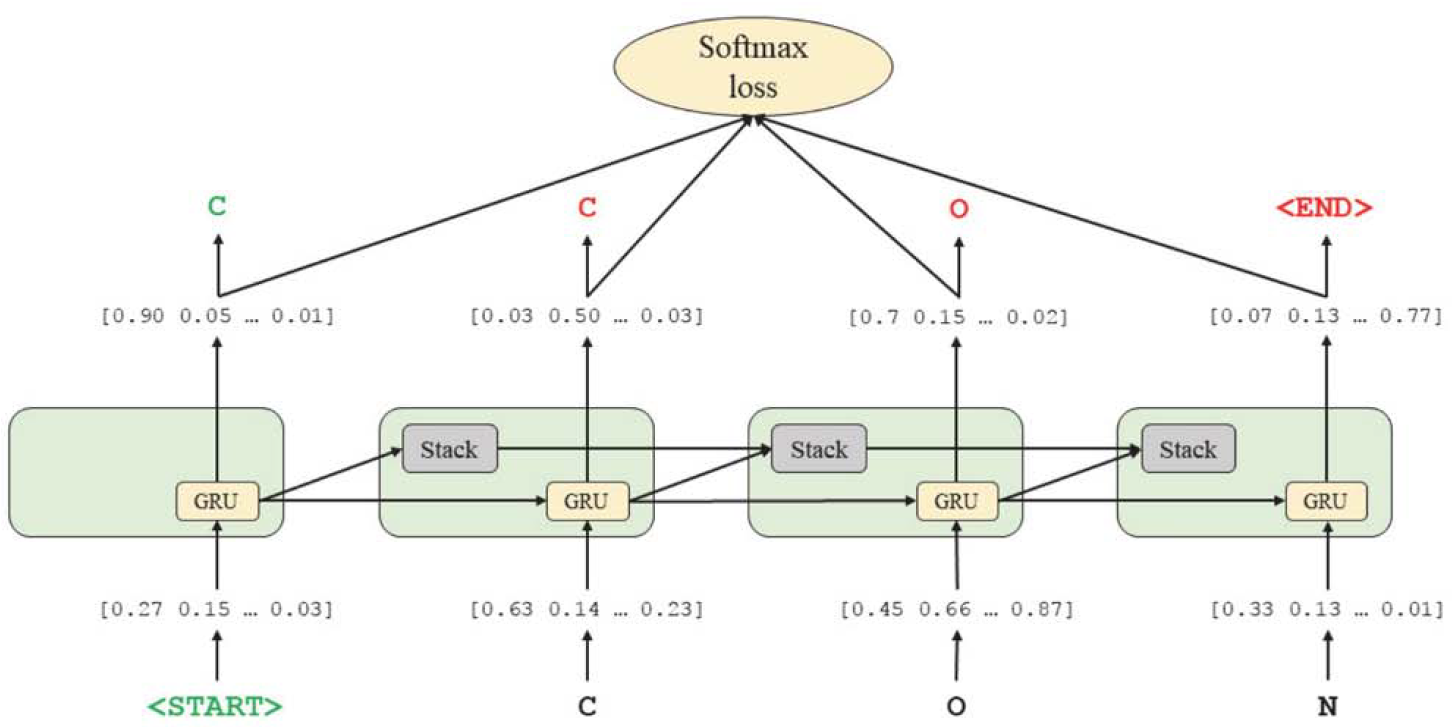
\includegraphics[width=0.50\textwidth]{softmax-loss.png}
		\caption{Training step of the generative Stack-RNN.}
		\label{fig:softmax-loss}
	\end{figure}
	
Then, the next character is sampled from this predicted probability distribution and is compared to the ground truth. Afterward, on the basis of this comparison, the cross-entropy loss function is calculated, and parameters of the model are updated. 
At each time step, in generating mode, the generative network takes a prefix of already generated sequences and then, like in the training mode, predicts the probability distribution of the next character and samples it from this predicted distribution (Fig. \ref{fig:predicted-distribution} - B). 

\begin{figure}[htbp]
		\centering
			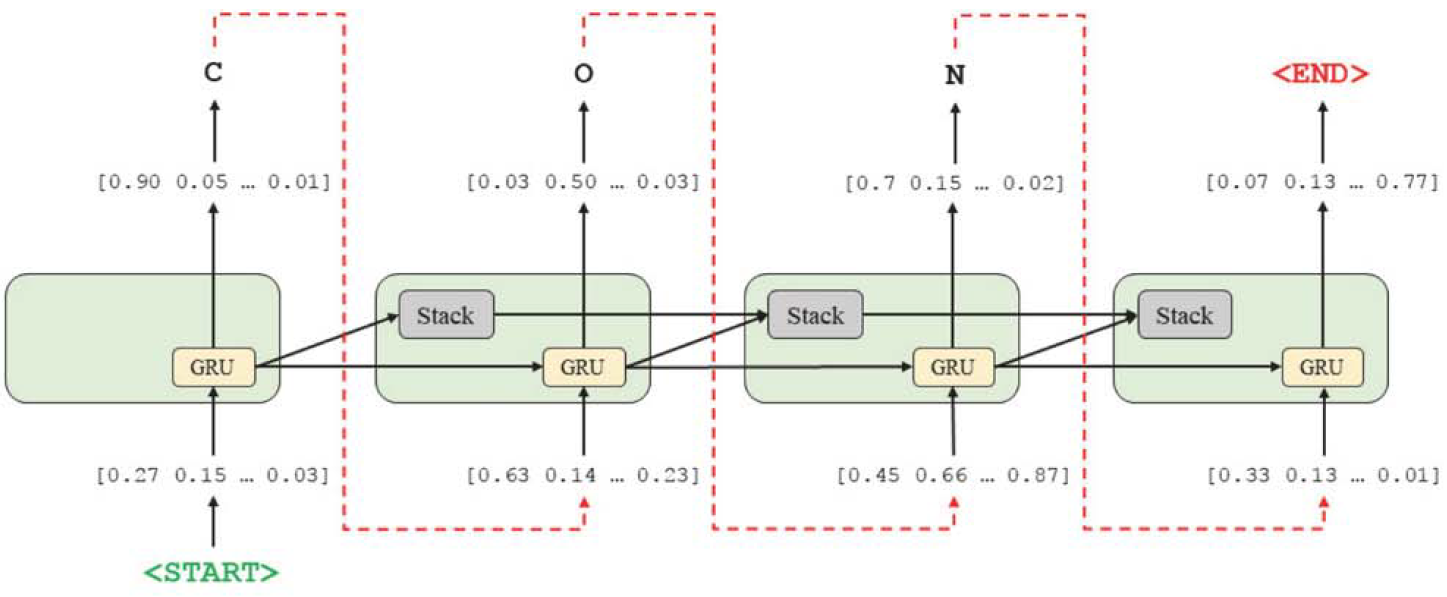
\includegraphics[width=0.50\textwidth]{predicted-distribution.png}
		\caption{Generator step of the generative Stack-RNN.}
		\label{fig:predicted-distribution}
	\end{figure}
	
In the generative model, the model parameters are not updated. 
At the second stage, both generative and predictive models are combined into one RL system, as shown in figure \ref{fig:parameter-optimization}. 

\begin{figure}[htbp]
		\centering
			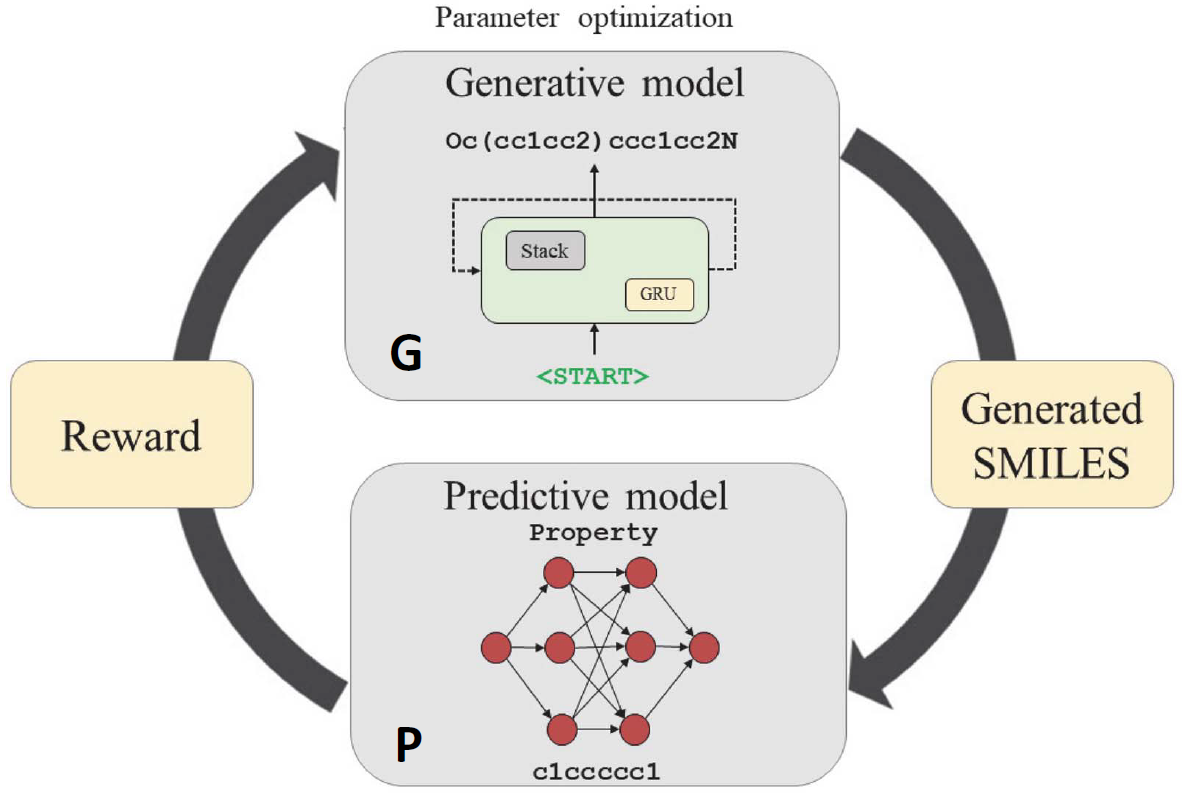
\includegraphics[width=0.50\textwidth]{parameter-optimization.png}
		\caption{General pipeline of RL system for novel compound generation.}
		\label{fig:parameter-optimization}
	\end{figure}

In this system, the generative model G (Fig. \ref{fig:parameter-optimization}) plays the role of an agent, whose action space is represented by the SMILES notation alphabet, and state space is represented by all possible strings in this alphabet.The predictive model plays the role of a critic estimating the agent’s behavior by assigning a numerical reward to every generated molecule (that is, SMILES string). 
The predictive model P (Fig. \ref{fig:parameter-optimization}) is a model for estimating physical, chemical, or biological properties of molecules. This property prediction model is a deep neural network, which consists of an embedding layer, an LSTM layer, and two dense layers. This network is designed to calculate user-specified property (activity) of the molecule taking a SMILES string as an input data vector. This model takes a SMILES string as an input and provides one real number, which is an estimated property value, as an output (Fig. \ref{fig:smiles-to-predicted-property}). In a practical sense, this learning step is analogous to traditional  quantitative structure–activity relationships (QSAR) models. However, unlike conventional QSAR, no numerical descriptors are needed, as the model distinctly learns directly from the SMILES notation as to how to relate the comparison between SMILES strings to that between target properties. The predictor uses, as shown in the figure \ref{fig:smiles-to-predicted-property}, two unidirectional LSTM layers with hidden size of 128 each, with an embedding size of 128. The dense layer is a Multi-layer Perceptron with hidden size of 128 and ReLU activation function.

\begin{figure}[htbp]
		\centering
			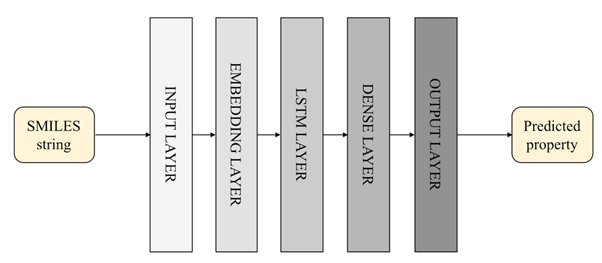
\includegraphics[width=0.50\textwidth]{smiles-to-predicted-property.png}
		\caption{Scheme of predictive model.}
		\label{fig:smiles-to-predicted-property}
	\end{figure}
	
The reward (Fig. \ref{fig:parameter-optimization}) is a function of the numerical property calculated by the predictive model. At this stage, the generative model is trained to maximize the expected reward.
The absolute majority of compounds generated de novo by the ReLeaSE method are novel structures as compared to the data sets used to train generative models, and any traditional quantitative structure–activity relationships model could be used to evaluate their properties.
As a proof of principle, the method has been tested on three diverse types of endpoints: physical properties, biological activity, and chemical substructure bias. The use of a flexible reward function enables different library optimization strategies where one can minimize,maximize, or impose a desired range to a property of interest in the generated compound libraries.

\section{The execution}\label{sec:The execution}

In this experiment we will optimize parameters of pretrained generative RNN to produce molecules with values of logP within drug-like regions according to Lipinsky rule. We use policy gradient algorithm with custom reward function to bias the properties of generated molecules.
The following example uses real SMILES strings, contained in a given input file (we used the ChEMBL database of drug-like compounds).
In this execution the generator produces a new SMILES string, which is then evaluated by the predictor. Based on the obtained prediction and the goal, it is assigned a numerical reward value and updated the parameters of the generator using policy gradient algorithm.
 
The policy gradient loss is defined as follow:

\begin{figure}[htbp]
		\centering
			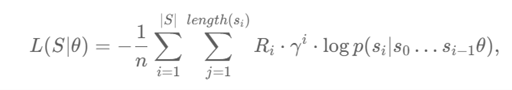
\includegraphics[width=0.50\textwidth]{formula.png}
		\label{fig:formula}
	\end{figure}

where \textit{R} is the reward obtained at time step i. \begin{math}\gamma\end{math} is the discount factor and \begin{math} p(s_i | s_1,\cdots ,s_i_-_1,\theta) \end{math} is the probability of the next character given the prefix, which is obtained from the generator. The reward is the same for every time step and is equal to the reward for the whole molecule. 

\section{Prerequisites}\label{sec:Prerequisites}

\mypar{Hardware}
Linux OS or WSL 2 on a Windows 10 (or higher) machine.
A Modern NVIDIA GPU, compatible with CUDA 11.3.

\mypar{Docker and Docker Compose}
Docker and Docker Compose (Application containers engine) are required; they can be installed from \href{https://www.docker.com}{here}.
The GPU Support is enabled on the machine; check it out \href{https://docs.docker.com/compose/gpu-support/}{here} 

\mypar{Nvidia Container Toolkit}
The Nvidia Container Toolkit is required; it can be installed from \href{https://docs.nvidia.com/datacenter/cloud-native/container-toolkit/install-guide.html#install-guide}{here}.
Note that you do not need to install the CUDA Toolkit on the host system.
Note that you have to install the NVIDIA drivers on your system.

\section{Installation}\label{sec:Installation}

In this section is described how to implement and run the ReLeaSe method on a machine.

\subsection{Instructions}\label{sec:Instructions}

As mentioned into the \href{https://github.com/IvanBuccella/SF2Bio#installation}{repository} of the project, the following instructions need to be performed for running the container:

\begin{lstlisting}
\$ git clone https://github.com/IvanBuccella/SF2Bio
HTTP_PORT=8888
\$ docker-compose build
\$ docker-compose up
\end{lstlisting}

\subsection{The Dockerfile}\label{sec:The Dockerfile}

During the installation and initialization phases of the project, some changes had to be made to the code to resolve errors that prevented it from starting. This could have been caused by several factors, such as the presence of outdated dependencies or incompatible package versions. These changes allowed the use of newer versions of the packages, which were more stable and compatible with the code. 
The result of this phase gave in output the construction of the Dockerfile which replicates the installation methodology described in the ReLeaSe method \href{https://github.com/isayev/ReLeaSE#installation-with-anaconda}{repository}. 

\begin{lstlisting}
1 FROM nvidia/cuda:11.3.0-cudnn8-runtime-ubuntu20.04

2 RUN apt-get update
3 RUN apt-get install -y git
4 RUN apt-get install -y wget

5 RUN wget https://repo.anaconda.com/miniconda/ Miniconda3-latest-Linux-x86_64.sh
6 RUN bash Miniconda3-latest-Linux-x86_64.sh -b -p /miniconda
7 ENV PATH=\$PATH:/miniconda/pcondabin:/miniconda/bin

8 RUN conda update -n base -c defaults conda
9 RUN conda create -n release python=3.6

10 SHELL ["conda","run","-n","release","/bin/bash", "-c"]

11 COPY environment environment
12 RUN conda install --yes --file environment/conda.txt
13 RUN conda install -c rdkit rdkit nox cairo
14 RUN conda install pytorch=1.10.1 torchvision=0.11.2 -c pytorch -c conda-forge
15 RUN pip install -r environment/pip.txt

16 WORKDIR /home

17 RUN git clone https://github.com/isayev/ReLeaSE.git .

18 ENTRYPOINT ["conda", "run", "-n", "release", "jupyter", "notebook", "--ip=0.0.0.0", "--port=8888", "--allow-root", "--NotebookApp.token=''", "--NotebookApp.password=''"]
\end{lstlisting}

As shown in the code above, build starts from the official \href{https://hub.docker.com/r/nvidia/cuda}{Nvidia CUDA docker image} with Ubuntu 20.04. To the initial image, several dependencies are added, like \href{https://docs.conda.io/en/latest/miniconda.html}{MiniConda} which is a bootstrap version of Anaconda [Row 5 del codice].
Once Conda is installed, a new environment with Python is created [Row 11 del codice] and the required dependencies specified in the conda.txt file are installed [Row 12 del codice]. In addition, RDKit, Nox, Cairo, pytorch and torchvision are installed [Rows 13-14 del codice]. 
Then the pip dependencies listed in the pip.txt file, such as \href{https://www.tensorflow.org/tensorboard}{tensorboard}, \href{https://www.tensorflow.org/}{tensorflow} are installed [Row 15 del codice].
Finally, the ReLeaSe code repository is cloned into the workdir of the image and the entrypoint of the jupyter notebook is defined.

\subsection{The Docker Compose}\label{sec:The Docker Compose}

\begin{lstlisting}
version: "3.8"

services:
  app:
    platform: linux/amd64
    build:
      context: .
      dockerfile: Dockerfile
    environment:
      - NVIDIA_DISABLE_REQUIRE=1
    ports:
      - \${HTTP_PORT}:8888
    deploy:
      resources:
        reservations:
          devices:
            - capabilities: [gpu]
\end{lstlisting}

As shown in the code above, the docker-compose file includes the GPU access \cite{gpu-support} to the service container “app” including all the nvidia GPUs installed on the host machine. This access allows the container to use the nvidia GPUs shared for the execution; in particular this allows “pytorch” to find and to use the CUDA cores.

\subsection{The running container}\label{sec:The running container}

\begin{figure}[htbp]
		\centering
			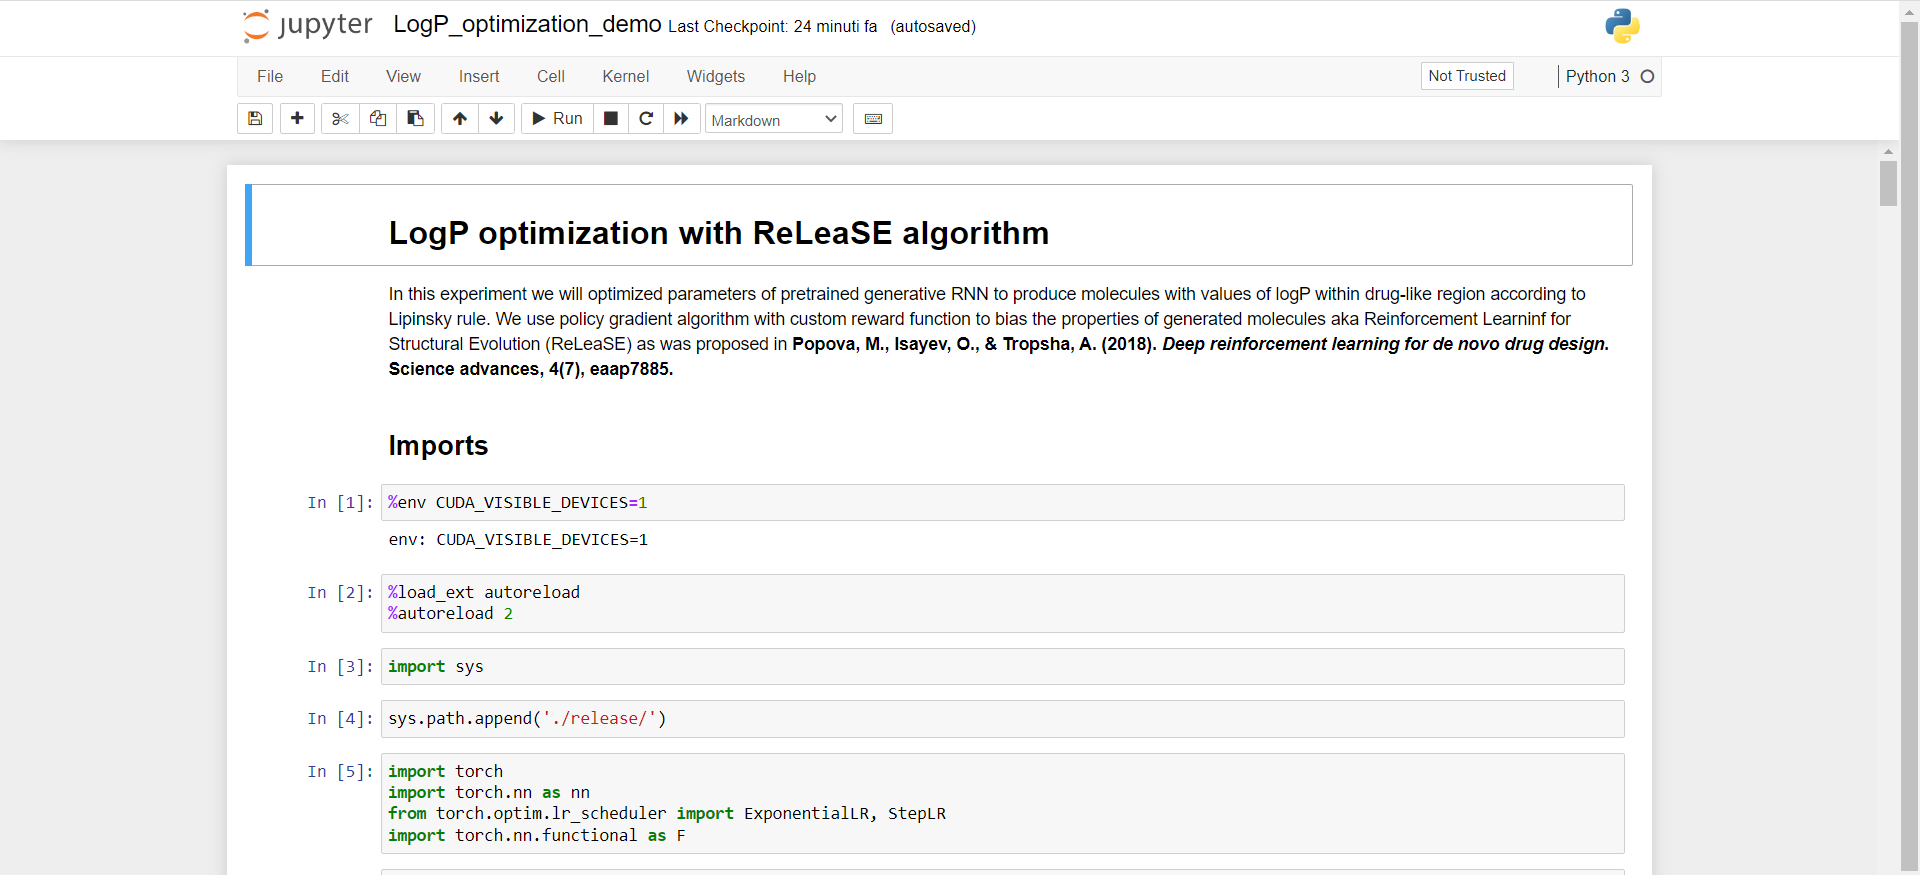
\includegraphics[width=0.50\textwidth]{logp-optimization.png}
		\label{fig:logp-optimization}
	\end{figure}

In the figure above is reported the configured jupyter notebook of the execution described in the following sections; it can be reached by visiting the \href{http://localhost:{HTTP_PORT}/LogP_optimization_demo.ipynb}{URL} into the host machine web browser.


\begin{comment}
\mypar{Loop interchange}
The first step is editing the starting algorithm by exchanging the order of the iteration variables \textbf{x} and \textbf{y} used by nested loops. The result is two different algorithms:

\setcounter{lstlisting}{0}
\renewcommand{\lstlistingname}{Algorithm}

\begin{lstlisting}[caption={The starting algorithm},label={lst:loop-interchange-x-y}]
for (x = 1; x < N - 1; x++)
{
		for (y = 1; y < N - 1; y++)
		{
				B[x][y] = a * A[x][y] + b * (A[x - 1][y] + A[x + 1][y] + A[x][y - 1] + A[x][y + 1]);
		}
}
\end{lstlisting}

\begin{lstlisting}[caption={A new algorithm with x and y swapped},label={lst:loop-interchange-y-x}]
for (y = 1; y < N - 1; y++)
{
		for (x = 1; x < N - 1; x++)
		{
				B[x][y] = a * A[x][y] + b * (A[x - 1][y] + A[x + 1][y] + A[x][y - 1] + A[x][y + 1]);
		}
}
\end{lstlisting}

\mypar{Optimization flags}
The next step is editing the optimization flag used for compiling the source code; the clang compiler offers four different flag specifications: O0, O1, O2, and O3. The result is four different commands:

\setcounter{lstlisting}{0}
\renewcommand{\lstlistingname}{Command}

\begin{lstlisting}[caption={Flag -O0},label={lst:optimization-flags-0}]
clang code.c -o code.out -fopenmp -O0
\end{lstlisting}

\begin{lstlisting}[caption={Flag -O1},label={lst:optimization-flags-1}]
clang code.c -o code.out -fopenmp -O1
\end{lstlisting}

\begin{lstlisting}[caption={Flag -O2},label={lst:optimization-flags-2}]
clang code.c -o code.out -fopenmp -O2
\end{lstlisting}

\begin{lstlisting}[caption={Flag -O3},label={lst:optimization-flags-3}]
clang code.c -o code.out -fopenmp -O3
\end{lstlisting}

\mypar{Parallel Loops}
The next step is editing the code by applying the parallel loops optimization. In order to distribute the execution of a loop into multiple threads, it has been used the ``#pragma omp parallel for'' \cite{omp-parallel}\cite{omp-for} directive; this directive opens a parallel region and schedules the loop into multiple threads. The directive could be applied to each loop, also on both. To apply the directive on both loops, it has been used the ``#pragma omp parallel for collapse(2)'' \cite{omp-collapse} directive which is able to distribute two nested loops on multiple threads. The result of this step is three different algorithms:

\setcounter{lstlisting}{2}
\renewcommand{\lstlistingname}{Algorithm}

\begin{lstlisting}[caption={Parallel loop on X},label={lst:parallel-loop-x}]
#pragma omp parallel for
for (x = 1; x < N - 1; x++)
{
		for (y = 1; y < N - 1; y++)
		{
				B[x][y] = a * A[x][y] + b * (A[x - 1][y] + A[x + 1][y] + A[x][y - 1] + A[x][y + 1]);
		}
}
\end{lstlisting}

\begin{lstlisting}[caption={Parallel loop on Y},label={lst:parallel-loop-y}]
for (x = 1; x < N - 1; x++)
{
		#pragma omp parallel for
		for (y = 1; y < N - 1; y++)
		{
				B[x][y] = a * A[x][y] + b * (A[x - 1][y] + A[x + 1][y] + A[x][y - 1] + A[x][y + 1]);
		}
}
\end{lstlisting}

\begin{lstlisting}[caption={Parallel loop on X and Y},label={lst:parallel-loop-x-y}]
#pragma omp parallel for collapse(2)
for (x = 1; x < N - 1; x++)
{
		for (y = 1; y < N - 1; y++)
		{
				B[x][y] = a * A[x][y] + b * (A[x - 1][y] + A[x + 1][y] + A[x][y - 1] + A[x][y + 1]);
		}
}
\end{lstlisting}

\mypar{Loop tiling}
The next step is editing the code by applying tiling optimization. In order to apply this type of optimization it has been necessary to cut the \textbf{A} matrix into multiple smaller \textit{tiles}; For this a new variable has been introduced into the code ``tile\textunderscore size'' which expresses the tile size, and two nested loops that have the goal of executing the code on the different tiles. On the tiling loops (with \textit{xx} and \textit{yy} variables) it has been applied the ``#pragma omp parallel for collapse(2)'' directive in order to distribute the matrices tiles on multiple threads. Different tile sizes have been chosen depending on several points of view like L2 Cache size, etc. The result of this step is four different algorithms, identical but with different tile sizes:

\renewcommand{\lstlistingname}{Algorithm}

\begin{lstlisting}[caption={Loop tiling with size of 16384},label={lst:tiling-1}]
const int tile_size = 16384;
#pragma omp parallel for collapse(2)
for (int xx = 0; xx < N; xx += tile_size)
{
		for (int yy = 0; yy < N; yy += tile_size)
		{
				for (x = xx + 1; x < MIN(xx + tile_size, N - 1); x++)
				{
						for (y = yy + 1; y < MIN(yy + tile_size, N - 1); y++)
						{
								B[x][y] = a * A[x][y] + b * (A[x - 1][y] + A[x + 1][y] + A[x][y - 1] + A[x][y + 1]);
						}
				}
		}
}
\end{lstlisting}

\begin{lstlisting}[caption={Loop tiling with size of 10922},label={lst:tiling-2}]
const int tile_size = 10922;
...same as before
\end{lstlisting}

\begin{lstlisting}[caption={Loop tiling with size of 8192},label={lst:tiling-3}]
const int tile_size = 8192;
...same as before
\end{lstlisting} 

\begin{lstlisting}[caption={Loop tiling with size of 5461},label={lst:tiling-4}]
const int tile_size = 5461;
...same as before
\end{lstlisting}

\mypar{Dimension augmentation}
The next step is editing the \textit{tiled} code by applying two more dimensions to the original Stencil code. In order to apply this step, it has been necessary to edit the internal loops (with \textit{x} and \textit{y} variables) condition from ``MIN(xx + tile\textunderscore size, N - 1)'' to ``MIN(xx + tile\textunderscore size, N - 3)''. Because of the tiling optimization, the code has been executed on different tile sizes depending on several points of view like L2 Cache size, etc. The result of this step is four different algorithms, identical but with different tile sizes:

\renewcommand{\lstlistingname}{Algorithm}

\begin{lstlisting}[caption={Dimension augmentation + loop tiling with size of 16384},label={lst:augmentation-1}]
const int tile_size = 16384;
#pragma omp parallel for collapse(2)
for (int xx = 0; xx < N; xx += tile_size)
{
		for (int yy = 0; yy < N; yy += tile_size)
		{
				for (x = xx + 3; x < MIN(xx + tile_size, N - 3); x = x + 3)
				{
						for (y = yy + 3; y < MIN(yy + tile_size, N - 3); y = y + 3)
						{
								B[x][y] = a * A[x][y] + b * (A[x - 3][y] + A[x - 2][y] + A[x - 1][y] + A[x + 1][y] + A[x + 2][y] + A[x + 3][y] + A[x][y - 3] + A[x][y - 2] + A[x][y - 1] + A[x][y + 1] + A[x][y + 2] + A[x][y + 3]);
						}
				}
		}
}
\end{lstlisting}

\begin{lstlisting}[caption={Dimension augmentation + loop tiling with size of 10922},label={lst:augmentation-2}]
const int tile_size = 10922;
...same as before
\end{lstlisting}

\begin{lstlisting}[caption={Dimension augmentation + loop tiling with size of 8192},label={lst:augmentation-3}]
const int tile_size = 8192;
...same as before
\end{lstlisting} 

\begin{lstlisting}[caption={Dimension augmentation + loop tiling with size of 5461},label={lst:augmentation-4}]
const int tile_size = 5461;
...same as before
\end{lstlisting}

\section{Experimental Results}\label{sec:exp}

\mypar{Experimental setup} The execution timing is obtained by using the OpenMP primitives \cite{omp-get-wtime}, an example is shown in Algorithm \ref{lst:omp-get-time-alg}. The OpenMP settings are shown in Algorithm \ref{lst:omp-configs-alg}. The experiment is executed on two matrices, A and B (initialized with the Algorithm \ref{lst:initialization-alg}), with a size of constant \textbf{N = 32768} and on a PC with current specifications: 
\begin{itemize}
	\item \textbf{CPU}
	\begin{itemize}
		\item \textbf{Model name}: Intel(R) Core(TM) i5-9600K CPU @ 3.70GHz
		\item \textbf{CPU(s)}: 6
		\item \textbf{Socket(s)}: 1
		\item \textbf{Core(s) per socket}: 6
		\item \textbf{Thread(s) per core}: 1
		\item \textbf{Cache L1d}: 192 KiB (6 instances)
		\item \textbf{Cache L1i}: 192 KiB (6 instances)
		\item \textbf{Cache L2}: 1.5 MiB (6 instances)
		\item \textbf{Cache L3}: 9 MiB (1 instance)
		\item \textbf{Intel Hyper-Threading Technology}: No
	\end{itemize}
	\item \textbf{Memory} 
	\begin{itemize}
		\item \textbf{Size}: 26164116 kB
	\end{itemize}
	\item \textbf{Compiler}: clang 14.0.5 with OpenMP 5.0
	\end{itemize}
\end{itemize}

\renewcommand{\lstlistingname}{Algorithm}

\begin{lstlisting}[caption={An example of code for obtaining the execution timing},label={lst:omp-get-time-alg}]
double t_init = omp_get_wtime()
//Your code's here
printf("\%0.15f", omp_get_wtime() - t_init);
\end{lstlisting}

\begin{lstlisting}[caption={OpenMP Configs},label={lst:omp-configs-alg}]
int n_threads = omp_get_max_threads();
omp_set_max_active_levels(1);
omp_set_num_threads(n_threads);
omp_set_dynamic(0);
\end{lstlisting}

\begin{lstlisting}[caption={A and B matrices initialization},label={lst:initialization-alg}]
float **A = (float **)malloc(N * sizeof(float *));
float **B = (float **)malloc(N * sizeof(float *));
for (x = 0; x < N; x++)
{
		A[x] = (float *)malloc(N * sizeof(float));
		B[x] = (float *)malloc(N * sizeof(float));
		for (y = 0; y < N; y++)
		{
				A[x][y] = 1.0f;
				B[x][y] = 0.0f;
		}
}
\end{lstlisting}

\mypar{Results}
Here the following execution timings are represented for every experiment that has been done.

\begin{itemize}
	\item \textbf{Loop interchange} computation time of: 
	\begin{itemize}
		\item the Algorithm \ref{lst:loop-interchange-x-y} is: 5.0533 (s) 
		\item the Algorithm \ref{lst:loop-interchange-y-x} is: 55.8343 (s)
	\end{itemize}
	\begin{figure}[htbp]
		\centering
			\includegraphics[width=0.50\textwidth]{loop-interchange.png}
		\caption{Loop interchange computation timings}
		\label{fig:loop-interchange}
	\end{figure}
	\item \textbf{Optimization flags}:
	\begin{itemize}
		\item the Algorithm \ref{lst:loop-interchange-x-y} by compiling with the command \ref{lst:optimization-flags-0} is: 5.0493 (s)
		\item the Algorithm \ref{lst:loop-interchange-x-y} by compiling with the command \ref{lst:optimization-flags-1} is: 1.3734 (s)
		\item the Algorithm \ref{lst:loop-interchange-x-y} by compiling with the command \ref{lst:optimization-flags-2} is: 0.5931 (s)
		\item the Algorithm \ref{lst:loop-interchange-x-y} by compiling with the command \ref{lst:optimization-flags-3} is: 0.5904 (s)
	\end{itemize}
	\begin{figure}[htbp]
		\centering
			\includegraphics[width=0.50\textwidth]{optimization-flags.png}
		\caption{Optimization flags computation timings}
		\label{fig:optimization-flags}
	\end{figure}	
	\item \textbf{Parallel loops}: 
	\begin{itemize}
		\item the Algorithm \ref{lst:parallel-loop-x} is: 0.4585 (s)
		\item the Algorithm \ref{lst:parallel-loop-y} is: 0.4760 (s)
		\item the Algorithm \ref{lst:parallel-loop-x-y} is: 0.7419 (s)
	\end{itemize}
	\begin{figure}[htbp]
		\centering
			\includegraphics[width=0.50\textwidth]{parallel-loops.png}
		\caption{Parallel loops computation timings}
		\label{fig:parallel-loops}
	\end{figure}		
	\item \textbf{Loop tiling}: 
	\begin{itemize}
		\item the Algorithm \ref{lst:tiling-1} is: 0.4451 (s)
		\item the Algorithm \ref{lst:tiling-2} is: 0.4599 (s)
		\item the Algorithm \ref{lst:tiling-3} is: 0.4422 (s)
		\item the Algorithm \ref{lst:tiling-4} is: 0.4537 (s)
	\end{itemize}	
	\begin{figure}[htbp]
		\centering
			\includegraphics[width=0.50\textwidth]{loop-tiling.png}
		\caption{Loop tiling computation timings}
		\label{fig:loop-tiling}
	\end{figure}		
	\item \textbf{Dimension augmentation}: 
	\begin{itemize}
		\item the Algorithm \ref{lst:augmentation-1} is: 0.2649 (s)
		\item the Algorithm \ref{lst:augmentation-2} is: 0.2911 (s)
		\item the Algorithm \ref{lst:augmentation-3} is: 0.2645 (s)
		\item the Algorithm \ref{lst:augmentation-4} is: 0.2676 (s)
	\end{itemize}	
	\begin{figure}[htbp]
		\centering
			\includegraphics[width=0.50\textwidth]{dimension-augmentation.png}
		\caption{Dimension augmentation computation timings}
		\label{fig:dimension-augmentation}
	\end{figure}
\end{itemize}

\section{Conclusions}
This article presents a number of different approaches to optimize the above-detailed Stencil computation's algorithm on multi-core architectures, based on a range of micro benchmarks.
For the \textbf{loop interchange} optimization, it indicates that the standard loop \textit{x-y} is faster than the \textit{y-x} loop, this is favored by the C programming language memory layout.
For the \textbf{optimization flags} optimization, it indicates that the best flag to use to compile the code is the -O3.
For the \textbf{parallel loop} optimization, it indicates that having only one parallel loop on the external loop is faster.
For the \textbf{loop tiling} optimization, it indicates that having a \textit{tile\textunderscore size} of \textit{8192} is faster.
About the \textbf{dimension} of the Stencil computation algorithm, it shows that by augmenting the number of dimensions of two, the computation is faster with \textbf{loop tiling} optimization than having a lower number of dimensions. In the table \ref{table:optimization-summary} is shown a summary with the best running time, relative and absolute speedups for every code optimization.

\renewcommand{\tablename}{Table}

\begin{table}[h!]
\begin{tabular}{||l r r r||} 
\hline
 Implementation & Running time & Rel. speedup & Abs. speedup \\ [0.5ex] 
 \hline\hline
 Starting algorithm & 5.0533 & 1.00 & 1.00 \\
 + Loop interchange & 5.0533 & 1.00 & 1.00 \\
 + Optimization flags & 0.5904 & 8.55 & 8.55 \\
 + Parallel loops & 0.4585 & 1.28 & 11.02 \\
 + Loop tiling & 0.4422 & 1.03 & 11.42 \\
 Dimension Augmentation & 0.2645 & 1.67 & 19.10 \\ [1ex] 
\hline
\end{tabular}
\caption{Summary}
\label{table:optimization-summary}
\end{table}

In future work, it would be interesting to try to implement what is the maximum number of dimension augmentation that offers a lower computation timing.
\end{comment}

\begin{thebibliography}{1}

\begin{comment}
\bibitem{taflove}
A. Taflove. Computational electrodynamics: The finite-difference time-domain method. 1995.

\bibitem{smith}
G. Smith. Numerical Solution of Partial Differential Equations: Finite Difference Methods. Oxford University Press, 2004.

\bibitem{cong-huang-zou}
J. Cong, M. Huang, and Y. Zou. Accelerating fluid registration algorithm on multi-FPGA platforms. FPL, 2011.

\bibitem{cong-zou}
On the Transformation Optimization for Stencil Computation

\bibitem{su-zhang-mei}
Huayou Su *, Kaifang Zhang and Songzhu Mei. On the Transformation Optimization for Stencil Computation

\bibitem{cruz}
Cruz, R.D.L.; Araya-Polo, M. Algorithm 942: Semi-Stencil. ACM Trans. Math. Softw. 2014, 40, 1–39.

\bibitem{barigou}
Youcef Barigou. Acceleration of real-life stencil codes on GPUs. Hardware Architecture [cs.AR]. 2011.

\bibitem{lipinski-rule}
\href{https://en.wikipedia.org/wiki/Lipinski\%27s_rule_of_five}{Lipinski's rule of five}

\bibitem{holewinski-pouchet-sadayappan}
Justin Holewinski, Louis-Noël Pouchet, P. Sadayappan. High-Performance Code Generation for Stencil Computations on GPU Architectures.

\bibitem{techopedia}
\href{https://www.techopedia.com/definition/5305/multicore}{Multi-core}

\bibitem{openmp}
\href{https://www.openmp.org/}{OpenMP}

\bibitem{loop-interchange}
\href{https://en.wikipedia.org/wiki/Loop_interchange}{Loop interchange}

\bibitem{optimization-flags}
\href{https://gcc.gnu.org/onlinedocs/gcc/Optimize-Options.html}{Options That Control Optimization}
 
\bibitem{loop-tiling}
João M.P.Cardoso, José Gabriel F. Coutinho, Pedro C. Diniz. Chapter 5 - Source code transformations and optimizations. Embedded Computing for High Performance

\bibitem{omp-get-wtime}
\href{https://www.openmp.org/spec-html/5.0/openmpsu160.html}{omp\textunderscore get\textunderscore wtime() function}

\bibitem{omp-parallel} 
\href{https://www.openmp.org/specifications/}{OpenMP API 5 Specification. OMP Parallel.}

\bibitem{omp-for}
\href{https://www.openmp.org/specifications/}{OpenMP API 5 Specification. OMP For.}

\bibitem{omp-collapse}
\href{https://www.openmp.org/specifications/}{OpenMP API 5 Specification. Collapse.}
\end{comment}

\bibitem{simplified-molecular-input-line-entry-system}
\href{https://en.wikipedia.org/wiki/Simplified_molecular-input_line-entry_system/}{Simplified molecular-input line-entry system}

\bibitem{arxiv}
\href{http://arxiv.org/abs/1412.3555/}{J. Chung, C. Gulcehre, K. Cho, Y. Bengio, Empirical evaluation of gated recurrent neural networks on sequence modeling, (2014).}

\bibitem{gpu-support}
\href{https://docs.docker.com/compose/gpu-support/}{Docker GPU support}

\end{thebibliography}

\end{document}